\begin{figure}[htb]
	\begin{center}
		\begin{minipage}[b]{0.9\linewidth}
			\centering
			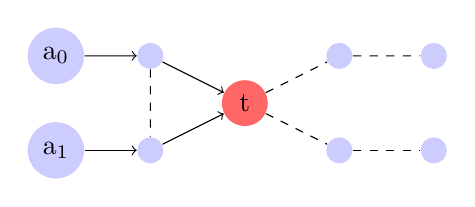
\begin{tikzpicture}
			  [scale=.6,auto=left,every node/.style={circle,fill=blue!20}]
			  \node (n1) at (1,3) {a$_0$};
			  \node (n2) at (3,3) { };
			  
	  		  \node (n3) at (1,1) {a$_1$};
			  \node (n4) at (3,1) { };
			  
			  \node[style={circle,fill=red!60}] (n5) at (5,2) {t};
			  
			  \node (n6) at (7,3) { };
			  \node (n7) at (7,1) { };
			  \node (n8) at (9,3) { };
			  \node (n9) at (9,1) { };
			  		  
			  \foreach \from/\to in {n1/n2,n2/n5,n3/n4,n4/n5}
			  \draw (\from) edge[->] (\to);
	
			  \foreach \from/\to in {n5/n6,n5/n7,n6/n8,n7/n9,n2/n4}
			  \draw (\from) edge[-,dashed] (\to);		  
			\end{tikzpicture}
			
			(a)\\
		\end{minipage}
		
		\bigskip
		\begin{minipage}[b]{0.9\linewidth}
			\centering
			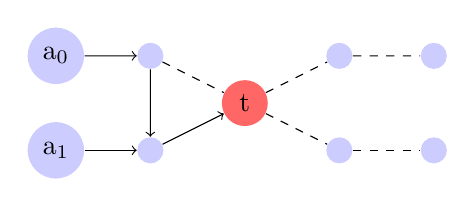
\begin{tikzpicture}
			  [scale=.6,auto=left,every node/.style={circle,fill=blue!20}]
			  \node (n1) at (1,3) {a$_0$};
			  \node (n2) at (3,3) { };
			  
	  		  \node (n3) at (1,1) {a$_1$};
			  \node (n4) at (3,1) { };
			  
			  \node[style={circle,fill=red!60}] (n5) at (5,2) {t};
			  
			  \node (n6) at (7,3) { };
			  \node (n7) at (7,1) { };
			  \node (n8) at (9,3) { };
			  \node (n9) at (9,1) { };
			  		  
			  \foreach \from/\to in {n1/n2,n3/n4,n4/n5,n2/n4}
			  \draw (\from) edge[->] (\to);
	
			  \foreach \from/\to in {n5/n6,n5/n7,n6/n8,n7/n9,n2/n5}
			  \draw (\from) edge[-,dashed] (\to);		  
			\end{tikzpicture}
			
			(b)\\
		\end{minipage}
	\end{center}
	\caption{\label{fig:prev_phi}
	     Ejemplos de emboscadas con dos agentes con valores de $\Phi$ de
	     $1.0$ para (a) dado que cubre dos caminos y $0.5$ para (b) dado que
	     cubre un camino. En el caso (b), se considera apenas un predecesor
	     del nodo $t$ de los dos predecesores posibles.
	}
\end{figure}